\begin{figure}[tbp] 
  \centering
  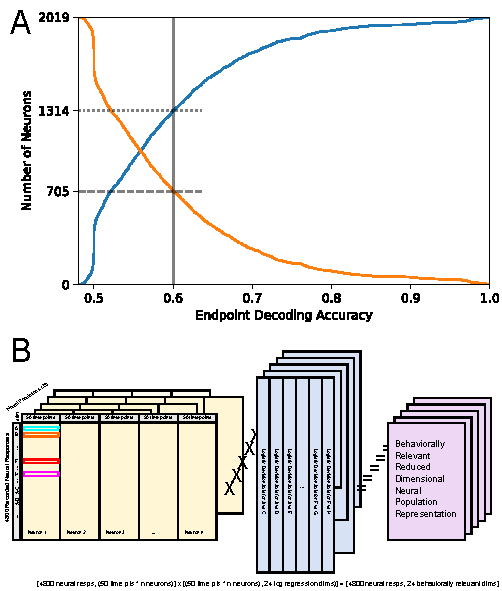
\includegraphics[width=85mm]{figures/fig06_neural_rep.pdf}
  \caption[Behaviorally relevant neural representation]
{
(A) The cumulative (blue) and survival (orange) curves for the distribution of units’ average accuracy on decoding pairs of the endpoint template motifs. The 0.6 accuracy cutoff was chosen mainly for computational tractability reasons. Subsequent analysis only includes activity of the 705 “behaviorally relevant neurons” with an average accuracy above 0.6. The 1314 neurons with average endpoint decoding accuracy below 0.6 were ignored by subsequent analysis.
(B) Diagram of the construction of the behaviorally relevant reduced dimensional neural population representation. We take the recorded neural representations from a population of “behaviorally relevant neurons”, sampled at 50 time points and concatenated to form a neural representation. We take the logistic decision axis for a logistic regression trained on the endpoints of the 24 morph dimensions to form the columns of a projection matrix which projects the neural population representation into 24 behaviorally relevant dimensions. The colored boxes correspond to the data which would be averaged to form the representations in the previous figure \ref{fig:single}. This behaviorally relevant neural representations are then used as the input to predict the Thielk curves (figure \ref{fig:derivative}) and and to predict the behavioral responses (figure \ref{fig:neurometric}). 
\index{neural_rep}}
  \label{fig:neural_rep}
\end{figure}